%iffalse
\let\negmedspace\undefined
\let\negthickspace\undefined
\documentclass[journal,12pt,onecolumn]{IEEEtran}
\usepackage[version=4]{mhchem}
\usepackage{chemformula} % for \ch if needed
\usepackage{chemfig}
\usepackage{chemmacros}
\chemsetup{modules = reactions} % Enables reaction arrows
\usepackage{graphicx}
\graphicspath{ {./images/} }
\usepackage{geometry}
\usepackage{lastpage}
\usepackage{cite}
\usepackage{amsmath,amssymb,amsfonts,amsthm}
\usepackage{enumitem,multicol}
\usepackage{algorithmic}
\usepackage{graphicx}
\usepackage{textcomp}
\usepackage{xcolor}
\usepackage{txfonts}
\usepackage{listings}
\usepackage{enumitem}
\usepackage{mathtools}
\usepackage{gensymb}
\usepackage{comment}
\usepackage[breaklinks=true]{hyperref}
\usepackage{tkz-euclide} 
\usepackage{listings}
\usepackage{gvv}                                        
%\def\inputGnumericTable{}                                 
\usepackage[latin1]{inputenc}                                
\usepackage{color}                                            
\usepackage{array}                                            
\usepackage{longtable}                                       
\usepackage{calc}                                             
\usepackage{multirow}                                         
\usepackage{hhline}                                           
\usepackage{ifthen}                                           
\usepackage{lscape}
\usepackage{tabularx}
\usepackage{array}
\usepackage{float}


\newtheorem{theorem}{Theorem}[section]
\newtheorem{problem}{Problem}
\newtheorem{proposition}{Proposition}[section]
\newtheorem{lemma}{Lemma}[section]
\newtheorem{corollary}[theorem]{Corollary}
\newtheorem{example}{Example}[section]
\newtheorem{definition}[problem]{Definition}
\newcommand{\BEQA}{\begin{eqnarray}}
\newcommand{\EEQA}{\end{eqnarray}}
\newcommand{\define}{\stackrel{\triangle}{=}}
\theoremstyle{remark}

\geometry{margin=1 in}



\setlength{\headheight}{14pt}
\setlength{\headsep}{5pt}
\setlength{\footskip}{20pt}
\begin{document}
1-5 carry one mark each
\begin{enumerate}


\item "You are delaying the completion of the task. Send  contributions at the earliest:"

\hfill{GATE 2023 PI}

\begin{multicols}{2}
\begin{enumerate}
    \item you are
    \item your
    \item you're
    \item yore
\end{enumerate}
\end{multicols}


\item References : \underline{\hspace{1.5cm}} : : Guidelines : Implement

(By word meaning)
\hfill{GATE 2023 PI}
\begin{multicols}{2}
\begin{enumerate}
    \item Sight
    \item Site
    \item Cite
    \item Plagiarise
\end{enumerate}
\end{multicols}
\item In the given figure, PQRS is a parallelogram with PS = 7 cm, PT = 4 cm and PV = 5 cm. What is the length of RS in cm? (The diagram is representative.)
\begin{figure}[H]
    \centering
    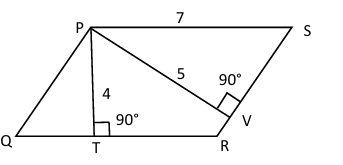
\includegraphics[width=0.5\linewidth]{figs/Q.1.png}
    \caption{fig1}
    \label{fig:figs/Q.1.png}
\end{figure}
\hfill{GATE 2023 PI}
\begin{multicols}{4}
    \begin{enumerate}
        \item 20/7
        \item 28/5
        \item 9/2
        \item 35/4
    \end{enumerate}
\end{multicols}
\item In 2022, June Huh was awarded the Fields medal, which is the highest prize in Mathematics.

When he was younger, he was also a poet. He did not win any medals in the International Mathematics Olympiads. He dropped out of college.

Based only on the above information, which one of the following statements can be logically inferred with certainty?

\begin{multicols}{2}
\begin{enumerate}
    \item Every Fields medalist has won a medal in an International Mathematics Olympiad.
    \item Everyone who has dropped out of college has won the Fields medal.
    \item All Fields medalists are part-time poets.
    \item Some Fields medalists have dropped out of college.
\end{enumerate}
\end{multicols}
\hfill{GATE 2023 PI}

\item A line of symmetry is defined as a line that divides a figure into two parts in a way such that each part is a mirror image of the other part about that line.

The given figure consists of 16 unit squares arranged as shown. In addition to the three black squares, what is the minimum number of squares that must be coloured black, such that both PQ and MN form lines of symmetry? (The figure is representative)
\begin{figure}[H]
    \centering
    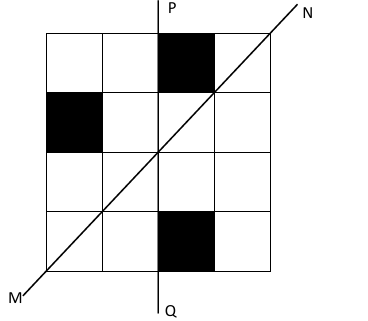
\includegraphics[width=0.5\linewidth]{figs/Q.5.png}
    \caption{fig2}
    \label{fig:figs/Q.5.png}
\end{figure}
\begin{multicols}{4}
    \begin{enumerate}
        \item 3
        \item 4
        \item 5
        \item 6
        \end{enumerate}
\end{multicols}
\item Human beings are one among many creatures that inhabit an imagined world. In this imagined world, some creatures are cruel. If in this imagined world, it is given that the statement "Some human beings are not cruel creatures" is FALSE, then which of the following set of statement(s) can be logically inferred with certainty?
\begin{enumerate}
    

     \item  All human beings are cruel creatures.
     \item  Some human beings are cruel creatures.
     \item Some creatures that are cruel are human beings.
     \item No human beings are cruel creatures.
\end{enumerate}
\hfill{GATE 2023 PI}

\begin{multicols}{2}
\begin{enumerate}
    \item only a
    \item only c and d
    \item only a and b
    \item a, b and c
\end{enumerate}
\end{multicols}


\item To construct a wall, sand and cement are mixed in the ratio of 3:1. The cost of sand and that of cement are in the ratio of 1:2.

If the total cost of sand and cement to construct the wall is 1000 rupees, then what is the cost (in rupees) of cement used?
\hfill{GATE 2023 PI}

\begin{multicols}{2}
\begin{enumerate}
    \item 400
    \item 600
    \item 800
    \item 200
\end{enumerate}
\end{multicols}
\item The World Bank has declared that it does not plan to offer new financing to Sri Lanka, which is battling its worst economic crisis in decades, until the country has an adequate macroeconomic policy framework in place. In a statement, the World Bank said Sri Lanka needed to adopt structural reforms that focus on economic stabilisation and tackle the root causes of its crisis. The latter has starved it of foreign exchange and led to shortages of food, fuel, and medicines. The bank is repurposing resources under existing loans to help alleviate shortages of essential items such as medicine, cooking gas, fertiliser, meals for children, and cash for vulnerable households.

Based only on the above passage, which one of the following statements can be inferred with certainty?

\hfill{GATE 2023 PI}

\begin{multicols}{2}
\begin{enumerate}
    \item According to the World Bank, the root cause of Sri Lanka's economic crisis is that it does not have enough foreign exchange.
    \item The World Bank has stated that it will advise the Sri Lankan government about how to tackle the root causes of its economic crisis.
    \item According to the World Bank, Sri Lanka does not yet have an adequate macroeconomic policy framework.
    \item The World Bank has stated that it will provide Sri Lanka with additional funds for essentials such as food, fuel, and medicines.
\end{enumerate}
\end{multicols}

\item The coefficient of \(x^4\) in the polynomial \((x-1)^3(x-2)^3\) is equal to \underline{\hspace{2cm}}.

\hfill{GATE 2023 PI}

\begin{multicols}{2}
\begin{enumerate}
    \item 33
    \item $-3$
    \item 30
    \item 21
\end{enumerate}
\end{multicols}
\item Which one of the following shapes can be used to tile (completely cover by repeating) a flat plane, extending to infinity in all directions, without leaving any empty spaces in between them? The copies of the shape used to tile are identical and are not allowed to overlap.

\hfill{GATE 2023 PI}

\begin{multicols}{2}
\begin{enumerate}
    \item circle
    \item regular octagon
    \item regular pentagon
    \item rhombus
\end{enumerate}
\end{multicols}
11-35 carry two marks each
\item Given matrices
\[
A = \begin{bmatrix}
1 & -1 & 4 \\
3 & 2 & -1 \\
2 & 1 & -1
\end{bmatrix}
\quad \text{and} \quad
B = \begin{bmatrix}
B_{11} & B_{12} & B_{13} \\
B_{21} & B_{22} & B_{23} \\
B_{31} & B_{32} & B_{33}
\end{bmatrix}
\]
$B$ is skew-symmetric matrix of $A$. $B_{13}$ is

\hfill{GATE 2023 PI}

\begin{multicols}{2}
\begin{enumerate}
    \item $-3$
    \item $-2$
    \item $2$
    \item $3$
\end{enumerate}
\end{multicols}

\item The non-linear differential equation from the following options is

\hfill{GATE 2023 PI}

\begin{multicols}{2}
\begin{enumerate}
    \item \( \frac{d^2y}{dx^2} + \frac{dy}{dx} + 10y = 0 \)
    \item \( \frac{d^2y}{dx^2} + \left(\frac{dy}{dx}\right)^2 + 10y = 0 \)
    \item \( \frac{d^2y}{dx^2} + \frac{dy}{dx} + 10x = 0 \)
    \item \( \frac{d^2y}{dx^2} + \frac{dy}{dx} + 10xy = 0 \)
\end{enumerate}
\end{multicols}
\item The power series expansion of a function is given as
\[
\frac{1}{x}\ln(1+x) = 1 + bx + cx^2 + \ldots
\]
for \(0 < x \leq 1\).

The values of constants \(b\) and \(c\), respectively, are

\hfill{GATE 2023 PI}

\begin{multicols}{2}
\begin{enumerate}
    \item $-\dfrac{1}{2}$ and $\dfrac{1}{3}$
    \item $\dfrac{1}{2}$ and $-\dfrac{1}{3}$
    \item $-1$ and $\dfrac{1}{2}$
    \item $1$ and $-\dfrac{1}{2}$
\end{enumerate}
\end{multicols}
\item Three unbiased coins are tossed. Provided that at least two outcomes are tails, the probability of having all three outcomes as tails is

\hfill{GATE 2023 PI}

\begin{multicols}{2}
\begin{enumerate}
    \item $\dfrac{1}{8}$
    \item $\dfrac{1}{4}$
    \item $\dfrac{1}{3}$
    \item $\dfrac{1}{2}$
\end{enumerate}
\end{multicols}

\item Two plane parallel surfaces exchange heat by thermal radiation. A radiation shield is placed in between at equal distance from the two surfaces to reduce heat transfer. All surfaces are black with infinite length and width. The ratio of heat transfer rate between surfaces with and without radiation shield is

\hfill{GATE 2023 PI}

\begin{multicols}{2}
\begin{enumerate}
    \item $\dfrac{1}{2}$
    \item $\dfrac{1}{4}$
    \item $\dfrac{1}{6}$
    \item $\dfrac{1}{8}$
\end{enumerate}
\end{multicols}
\item As per the ANSI marking system, a grinding wheel with alumina as abrasive is designated as

\textbf{51 \hspace{1em} A \hspace{1em} 36 \hspace{1em} \textbf{K} \hspace{1em} 5 \hspace{1em} V \hspace{1em} 23}

Here, \textbf{K} indicates that

\hfill{GATE 2023 PI}

\begin{multicols}{2}
\begin{enumerate}
    \item abrasive used in the wheel is aluminum oxide
    \item hardness of the wheel is medium
    \item bonding material of the wheel is shellac
    \item structure of the wheel is dense
\end{enumerate}
\end{multicols}
\item The combination of Directrix and Generatrix in a machining operation is shown in figure. The surface produced is

\hfill{GATE 2023 PI}
\begin{figure}[H]
    \centering
    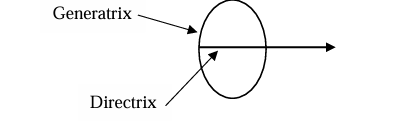
\includegraphics[width=0.25\linewidth]{figs/Q.17.png}
    \caption{fig3}
    \label{fig:figs/Q.17.png}
\end{figure}
\item In NC machine, the function of interpolator is to

\hfill{GATE 2023 PI}

\begin{multicols}{2}
\begin{enumerate}
    \item compute and maintain the tool feed rate
    \item compute and maintain the velocity of the slide
    \item generate warning signal based on the error
    \item generate reference signals prescribing the shape of the produced part
\end{enumerate}
\end{multicols}

\item Vacuum in the machining zone is an essential requirement for

\hfill{GATE 2023 PI}

\begin{multicols}{2}
\begin{enumerate}
    \item Electric Discharge Machining
    \item Chemical Machining
    \item Electro Chemical Machining
    \item Electron Beam Machining
\end{enumerate}
\end{multicols}
\item The qualitative method of forecasting amongst the given options is

\hfill{GATE 2023 PI}

\begin{multicols}{2}
\begin{enumerate}
    \item Linear Regression
    \item Weighted Moving Average
    \item Delphi
    \item Exponential Smoothing
\end{enumerate}
\end{multicols}

\item Transformation matrix to translate a point $P$ from $(10, 15)$ to $(15, 25)$ is

\hfill{GATE 2023 PI}

\begin{multicols}{2}
\begin{enumerate}
    \item $
    \begin{bmatrix}
    1 & 0 & 5 \\
    0 & 1 & 10 \\
    0 & 0 & 1
    \end{bmatrix}
    $
    \item $
    \begin{bmatrix}
    1 & 0 & 10 \\
    0 & 1 & 5 \\
    0 & 0 & 1
    \end{bmatrix}
    $
    \item $
    \begin{bmatrix}
    5 & 0 & 0 \\
    0 & 10 & 0 \\
    0 & 0 & 1
    \end{bmatrix}
    $
    \item $
    \begin{bmatrix}
    10 & 0 & 0 \\
    0 & 5 & 0 \\
    0 & 0 & 1
    \end{bmatrix}
    $
\end{enumerate}
\end{multicols}
\item A copper rod of 200 mm diameter and 400 mm length is extruded to the final diameter of 100 mm. The extrusion ratio is

\hfill{GATE 2023 PI}

\begin{multicols}{2}
\begin{enumerate}
    \item 1
    \item 2
    \item 4
    \item 8
\end{enumerate}
\end{multicols}

\item A symbol for surface texture parameters is shown in figure. The difference between maximum and minimum values of surface roughness ($R_a$) is
\begin{figure}
    \centering
    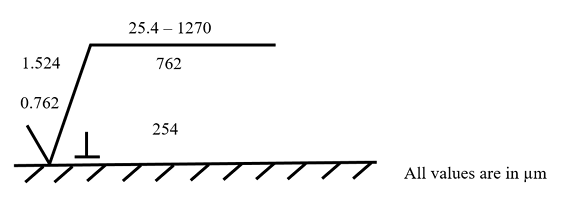
\includegraphics[width=0.5\linewidth]{figs/Q.23.png}
    \caption{fig4}
    \label{fig:figs/Q.23.png}
\end{figure}
\hfill{GATE 2023 PI}
\begin{multicols}{2}
\begin{enumerate}
    \item $0.499\,\mu\text{m}$
    \item $0.508\,\mu\text{m}$
    \item $0.762\,\mu\text{m}$
    \item $1.524\,\mu\text{m}$
\end{enumerate}
\end{multicols}

\item A thin cylinder has length $L$, diameter $d$, and thickness $t$. It is made of a material with modulus of elasticity $E$ and Poisson's ratio $\mu$. When the cylinder is subjected to an internal pressure $P$, the change in length is

\hfill{GATE 2023 PI}

\begin{multicols}{2}
\begin{enumerate}
    \item $\dfrac{PdL}{2tE}\left(\dfrac{1}{2} - \mu\right)$
    \item $\dfrac{PdL}{2tE}(2 - \mu)$
    \item $\dfrac{PdL}{2tE}(1 - 2\mu)$
    \item $\dfrac{PdL}{4tE}\left(\dfrac{1}{2} - \mu\right)$
\end{enumerate}
\end{multicols}

\item Creep of mild steel at elevated temperature involves

\hfill{GATE 2023 PI}

\begin{multicols}{2}
\begin{enumerate}
    \item elastic deformation under constant load
    \item elastic deformation under dynamic load
    \item plastic deformation under constant load
    \item plastic deformation under dynamic load
\end{enumerate}
\end{multicols}
\item Number of minimum control points required to generate a quadratic B-Spline curve is

\hfill{GATE 2023 PI}

\begin{multicols}{2}
\begin{enumerate}
    \item 2
    \item 4
    \item 8
    \item 16
\end{enumerate}
\end{multicols}

\item The Euler's method is used to solve
\[
\frac{dy}{dx} = x^3 y - 4, \; \; y(0) = 1
\]
The step size is 0.1. The approximate value of $y(0.1)$ is \underline{\hspace{2cm}} \textit{(round off to 2 decimal places)}.

\hfill{GATE 2023 PI}

\item A solid circular disk of 0.025 m thickness is used as flywheel. The density of the disk material is 7800 kg/m$^3$ and the mass moment of inertia of the disk about its center is 4.36 kg-m$^2$. The radius, in m, of the disk is \underline{\hspace{2cm}} \textit{(round off to 2 decimal places)}.

\hfill{GATE 2023 PI}
\item The standard time for completing a job on a machine is 10 minutes. Number of machines available is $5$, each machine is available for $300$ hours/month, and average machine utilization is $80$\%. The maximum number of jobs that can be produced in a month is \underline{\hspace{2cm}} \textit{(in integer)}.

\hfill{GATE 2023 PI}

\item Travel details of two persons P and Q travelling from city X to city Y are given as

\begin{center}
\begin{tabular}{|c|c|c|c|}
\hline
Person & Mode of travel & \begin{tabular}{c}
Monetary worth of functions\\
(travel time and comfort),\\
in Rupees
\end{tabular} & Ticket cost,\\
 &  &  & in Rupees\\
\hline
P & Aircraft & 8000 & 4000\\
Q & Train & 2000 & 2000\\
\hline
\end{tabular}
\end{center}

The positive difference in value of travel between the two modes is \underline{\hspace{2cm}} \textit{(in integer)}.

\hfill{GATE 2023 PI}

\item A wooden cubical block of side $0.1$ m has specific gravity (SG) of $0.75$. It is held submerged in a pool of oil and water by a massless rigid wire as shown in figure. The density of water is $1000$ kg/m$^3$ and acceleration due to gravity is $9.8$ m/s$^2$. The tension, in N, in the wire is \underline{\hspace{2cm}} \textit{(round off to 2 decimal places)}.

\hfill{GATE 2023 PI}


\begin{figure}[H]
    \centering
    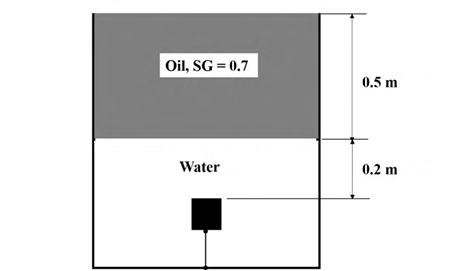
\includegraphics[width=0.5\linewidth]{figs/Q.31.png}
    \caption{fig5}
    \label{fig:figs/Q.31.png}
\end{figure}



\item Under steady state conditions, superheated steam enters the turbine with enthalpy, $h_1 = 3200$ kJ/kg and wet steam leaves the turbine at pressure $p_2 = 0.1$ bar. The heat loss is $100$ kJ/kg and work output is $1000$ kJ/kg. Kinetic and potential energies for inflow and outflow are neglected. At pressure 0.1 bar, the enthalpy of saturated liquid is $200$ kJ/kg and the enthalpy of vaporization is $2400$ kJ/kg. The dryness fraction of the steam at the exit of the turbine is \underline{\hspace{2cm}} \textit{(round off to 2 decimal places)}.

\hfill{GATE 2023 PI}
\item The total number of nonconformities is 420 from 30 samples. The size of each sample is 100. The lower control limit for the control chart for number of nonconformities is \underline{\hspace{2cm}} \textit{(round off to 2 decimal places)}.

\hfill{GATE 2023 PI}

\item Two metal sheets are joined using resistance spot welding. A welding current of 4500 A is applied for 0.2 s. The effective contact resistance at the sheet interface is $400 \times 10^{-6}\, \Omega$. The thermal efficiency of the welding process is 50\%. The amount of heat, in J, used for producing a spot weld is \underline{\hspace{2cm}} \textit{(in integer)}.

\hfill{GATE 2023 PI}

\item A metal rod of diameter 14 mm is subjected to a tensile test. After the test, its cross-sectional diameter at the fractured end is 12 mm. The ductility, in \%, is \underline{\hspace{2cm}} \textit{(round off to 2 decimal places)}.

\hfill{GATE 2023 PI}
\item Given, $z(x, y) = e^{x - 2y}$, where $x(t) = e^{t}$ and $y(t) = e^{-t}$. All the variables are real. The total differential $\dfrac{dz}{dt}$ is

\hfill{GATE 2023 PI}

\begin{multicols}{2}
\begin{enumerate}
    \item $-z(x + 2y)$
    \item $-z(x - 2y)$
    \item $z(x + 2y)$
    \item $z(x - 2y)$
\end{enumerate}
\end{multicols}

\item Two cards are drawn one after the other from a regular deck of $52$ playing cards without replacement. The probability that the drawn cards are of different suits is

\hfill{GATE 2023 PI}

\begin{multicols}{2}
\begin{enumerate}
    \item $\dfrac{39}{51}$
    \item $\dfrac{13}{52}$
    \item $\dfrac{2}{52}$
    \item $\dfrac{2}{51}$
\end{enumerate}
\end{multicols}

\item Match the machine elements with their functions.

\begin{center}
\begin{tabular}{|l|l|l|l|}
\hline
\textbf{Machine element} & & \textbf{Function} & \\
\hline
\textbf{P} & Collet         & \textbf{1} & Indexing \\
\textbf{Q} & Dividing head  & \textbf{2} & Thread cutting \\
\textbf{R} & Lead screw     & \textbf{3} & Holding the tool in place \\
\hline
\end{tabular}
\end{center}

\hfill{GATE 2023 PI}

\begin{multicols}{2}
\begin{enumerate}
    \item P -- 3, Q -- 2, R -- 1
    \item P -- 3, Q -- 1, R -- 2
    \item P -- 2, Q -- 1, R -- 3
    \item P -- 1, Q -- 3, R -- 2
\end{enumerate}
\end{multicols}
\item A massless beam is fixed at one end and supported on a roller at other end. A point force $P$ is applied at the midpoint of the beam as shown in figure. The reaction at the roller support is
\begin{figure}
    \centering
    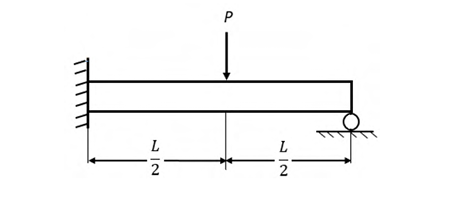
\includegraphics[width=0.5\linewidth]{figs/Q.39.png}
    \caption{fig6}
    \label{fig:figs/Q.39.png}
\end{figure}

\hfill{GATE 2023 PI}

\begin{multicols}{2}
\begin{enumerate}
    \item $\dfrac{5P}{16}$
    \item $\dfrac{2P}{3}$
    \item $\dfrac{4P}{9}$
    \item $\dfrac{9P}{25}$
\end{enumerate}
\end{multicols}
\item Six jobs (1, 2, 3, 4, 5, 6) undergo drilling, followed by reaming operation. The time required for each operation is given as

\begin{center}
\begin{tabular}{|c|c|c|}
\hline
\textbf{Job} & \textbf{Drilling (min)} & \textbf{Reaming (min)} \\
\hline
1 & 30 & 45 \\
2 & 30 & 15 \\
3 & 60 & 40 \\
4 & 20 & 25 \\
5 & 35 & 28 \\
6 & 45 & 70 \\
\hline
\end{tabular}
\end{center}

The sequence of processing the jobs, using the Johnson's rule, is

\hfill{GATE 2023 PI}

\begin{multicols}{2}
\begin{enumerate}
    \item 4 -- 1 -- 6 -- 3 -- 5 -- 2
    \item 4 -- 6 -- 1 -- 5 -- 3 -- 2
    \item 2 -- 1 -- 6 -- 3 -- 5 -- 4
    \item 2 -- 1 -- 3 -- 6 -- 5 -- 4
\end{enumerate}
\end{multicols}
\item Match the engineering materials at room temperature with the given crystal structures.

\begin{center}
\begin{tabular}{|l|l|l|l|}
\hline
\textbf{Engineering material} & & \textbf{Crystal structure} & \\
\hline
\textbf{P} & Si    & \textbf{1} & FCC \\
\textbf{Q} & Fe    & \textbf{2} & HCP \\
\textbf{R} & Al    & \textbf{3} & Diamond Cubic \\
\textbf{S} & Zn    & \textbf{4} & BCC \\
\hline
\end{tabular}
\end{center}

\hfill{GATE 2023 PI}

\begin{multicols}{2}
\begin{enumerate}
    \item P -- 3, Q -- 4, R -- 1, S -- 2
    \item P -- 2, Q -- 1, R -- 4, S -- 3
    \item P -- 2, Q -- 4, R -- 1, S -- 3
    \item P -- 3, Q -- 1, R -- 4, S -- 2
\end{enumerate}
\end{multicols}
\item Match the recording techniques used in method study with the most appropriate application areas.

\hfill{GATE 2023 PI}

\begin{multicols}{2}
\textbf{Recording technique}
\begin{enumerate}
    \item[(P)] Outline process chart
    \item[(Q)] String diagram
    \item[(R)] Multiple activity chart
    \item[(S)] Two-handed process chart
\end{enumerate}
\columnbreak
\textbf{Application area}
\begin{enumerate}
    \item[1.] Factory layout - movement of workers
    \item[2.] Gang work
    \item[3.] Complete manufacturing sequence of a product
    \item[4.] Manual assembly of nuts and bolts
\end{enumerate}
\end{multicols}

\begin{multicols}{2}
\begin{enumerate}
    \item P -- 3, Q -- 4, R -- 2, S -- 1
    \item P -- 3, Q -- 1, R -- 2, S -- 4
    \item P -- 2, Q -- 4, R -- 3, S -- 1
    \item P -- 2, Q -- 1, R -- 3, S -- 4
\end{enumerate}
\end{multicols}
\item Match the products to be manufactured with the given metal working processes.

\hfill{GATE 2023 PI}

\begin{multicols}{2}
\textbf{Product}
\begin{enumerate}
    \item[(P)] Beverage can
    \item[(Q)] Seamless pipe
    \item[(R)] Connecting rod
    \item[(S)] Steel balls for bearing
\end{enumerate}
\columnbreak
\textbf{Process}
\begin{enumerate}
    \item[1.] Forging
    \item[2.] Skew Rolling
    \item[3.] Extrusion
    \item[4.] Deep Drawing
\end{enumerate}
\end{multicols}

\begin{multicols}{2}
\begin{enumerate}
    \item P -- 3, Q -- 4, R -- 1, S -- 2
    \item P -- 2, Q -- 4, R -- 1, S -- 3
    \item P -- 4, Q -- 3, R -- 2, S -- 1
    \item P -- 4, Q -- 3, R -- 1, S -- 2
\end{enumerate}
\end{multicols}
\item The dual of a LPP is

\begin{equation*}
\text{Minimize}\ w = 4w_1 + 6w_2 + 5w_3 - w_4
\end{equation*}

subject to,
\begin{equation*}
\begin{bmatrix}
1 & 0 & 1 & 0 \\
0 & 0 & 1 & -1
\end{bmatrix}
\begin{bmatrix}
w_1 \\ w_2 \\ w_3 \\ w_4
\end{bmatrix}
\geq
\begin{bmatrix}
3 \\ -2
\end{bmatrix}
\end{equation*}

and $w_i \geq 0$ \quad for \quad $i = 1, 2, 3, 4$

The objective function of the primal is

\hfill{GATE 2023 PI}

\begin{multicols}{2}
\begin{enumerate}
    \item $\text{Maximize}\ z = -3x_1 + 2x_2$
    \item $\text{Maximize}\ z = x_1 + x_3$
    \item $\text{Maximize}\ z = x_3 - x_4$
    \item $\text{Maximize}\ z = 3x_1 - 2x_2$
\end{enumerate}
\end{multicols}
\item There are four locations (P, Q, R, S) and four factors to be considered for setting up a facility. The scores (on a scale of 0 to 10, with 10 being the maximum) for the given locations and the weight assigned to each factor are given as

\begin{center}
\begin{tabular}{|l|c|c|c|c|c|}
\hline
\textbf{Factor} & \textbf{Weight} & \textbf{P} & \textbf{Q} & \textbf{R} & \textbf{S} \\
\hline
Availability of raw material   & 0.4 & 6  & 8  & 5  & 4  \\
Availability of skilled labor  & 0.3 & 7  & 4  & 10 & 6  \\
Infrastructure                & 0.2 & 8  & 3  & 10 & 8  \\
Proximity to market           & 0.1 & 10 & 8  & 7  & 5  \\
\hline
\end{tabular}
\end{center}

The best location for setting up the facility is

\hfill{GATE 2023 PI}

\begin{multicols}{2}
\begin{enumerate}
    \item P
    \item Q
    \item R
    \item S
\end{enumerate}
\end{multicols}
\item As per the Fe-C phase diagram, the microstructure of plain carbon steel with 0.4 wt.\% carbon at room temperature contains

\hfill{GATE 2023 PI}

\begin{multicols}{2}
\begin{enumerate}
    \item proeutectoid ferrite and pearlite
    \item proeutectoid cementite and pearlite
    \item ferrite and austenite
    \item austenite and cementite
\end{enumerate}
\end{multicols}

\item The most appropriate process for manufacturing of plastic chair is

\hfill{GATE 2023 PI}

\begin{multicols}{2}
\begin{enumerate}
    \item injection molding
    \item extrusion
    \item calendering
    \item blow molding
\end{enumerate}
\end{multicols}
\item The following equation is solved using Newton-Raphson method
\[
x^5 - 15 = 0
\]
with initial value \( x_0 = 1.0 \).

The value of first approximation \( x_1 \) is \rule{3cm}{0.15mm} \textit{(round off to 2 decimal places).}

\hfill{GATE 2023 PI}

\item For the matrix 
\[
\begin{bmatrix}
4 & 2 \\
3 & 3
\end{bmatrix},
\]
eigenvalue corresponding to the eigenvector 
\(
\begin{bmatrix}
2 \\
-3
\end{bmatrix}
\)
is \rule{3cm}{0.15mm} \textit{(in integer).}

\hfill{GATE 2023 PI}

\item The work sampling study, with 100 observations, revealed 25\% idle time of a worker. The number of observations required for $\pm$10\% accuracy and 95.45\% confidence level is \rule{3cm}{0.15mm} \textit{(in integer).}

\hfill{GATE 2023 PI}
\item The information of two products P and Q is given as

\begin{center}
\begin{tabular}{|l|c|c|c|}
\hline
\textbf{Product} & \textbf{Annual demand (units)} & \textbf{Ordering cost per order (Rupees)} & \textbf{Holding cost per unit per year (Rupees)} \\
\hline
P & 2500 & 60 & 30 \\
Q & 3600 & 80 & 40 \\
\hline
\end{tabular}
\end{center}

The value of  
\[
\frac{\text{Economic Order Quantity of product P}}{\text{Economic Order Quantity of product Q}}
\]
is \rule{3cm}{0.15mm} \textit{(round off to 2 decimal places).}

\hfill{GATE 2023 PI}


\item A system shown in figure has seven components with reliabilities $R_A = 0.96$, $R_B = 0.92$, $R_C = 0.94$, $R_D = 0.89$, $R_E = 0.95$, $R_F = 0.88$, and $R_G = 0.90$. The reliability of the system is \rule{3cm}{0.15mm} \textit{(round off to 2 decimal places).}
\begin{figure}[H]
    \centering
    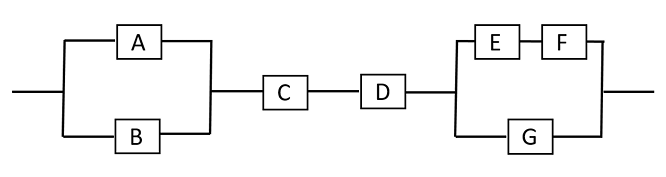
\includegraphics[width=0.5\linewidth]{figs/Q.54.png}
    \caption{fig7}
    \label{fig:figs/Q.54.png}
\end{figure}

\hfill{GATE 2023 PI}
\item Details of activities of a project are given as

\begin{center}
\begin{tabular}{|l|c|c|c|c|c|c|c|c|c|c|c|}
\hline
\textbf{Activity} & A & B & C & D & E & F & G & H & I & J \\
\hline
\textbf{Time (days)} & 8 & 10 & 8 & 7 & 16 & 15 & 18 & 14 & 9 & 4 \\
\hline
\textbf{Predecessors} & - & - & - & A & A & B, D & C & C & F, G & E, I, H \\
\hline
\end{tabular}
\end{center}

The time required, in days, to complete the project along the critical path is \rule{3cm}{0.15mm} \textit{(in integer).}

\hfill{GATE 2023 PI}


\item A system has 10 essential components. Each component has an exponential time-to-failure distribution with constant failure rate of $0.04$ per $4000$ hours.
The mean-time-to-failure, in hours, of the system is \rule{3cm}{0.15mm} \textit{(in integer).}

\hfill{GATE 2023 PI}


\item A CNC water jet cutting machine is used to cut a straight slot between the points $(2,\,1)$ and $(10,\,10)$ on the XY plane (dimensions are in mm). If the feed rate is $1.5$ mm/s, the time, in s, required to machine the slot following the shortest path, is \rule{3cm}{0.15mm} \textit{(round off to 2 decimal places).}

\hfill{GATE 2023 PI}


\item In an orthogonal cutting with a tool of rake angle $0^\circ$, the value of the cutting force is two times of the thrust force. The coefficient of friction is \rule{3cm}{0.15mm} \textit{(round off to 1 decimal place).}

\hfill{GATE 2023 PI}
\item The solidification of a cubical casting of side $100$ mm takes place with volumetric solidification shrinkage and solid contraction of $10\%$ each. The shape of the casting is retained on cooling to room temperature. The side of the cubical cast, in mm, at room temperature is \rule{3cm}{0.15mm} \textit{(round off to 2 decimal places).}

\hfill{GATE 2023 PI}

\item A straight turning operation is carried out at the feed rate of $100$ mm/min using a single point cutting tool with signature $8-8-5-5-7-25-0$ (ASA). The spindle speed is $1600$ rpm. The roughness, in $\mu$m, of the machined surface in terms of peak-to-valley height is \rule{3cm}{0.15mm} \textit{(round off to 2 decimal places).}

\hfill{GATE 2023 PI}

\item An arc welding operation is performed at $25$ V and $200$ A at welding speed of $2$ mm/s. The heat used for melting is $80\%$ of the total heat generated. The unit melting energy of the metal to be joined is $10$ J/mm$^3$. The volume of the weld metal produced per unit time, in mm$^3$/s, is \rule{3cm}{0.15mm} \textit{(in integer).}

\hfill{GATE 2023 PI}

\item Water flows through a pipe of diameter $0.02$ m. The Reynolds number of the flow is $1000$. The pipe is heated from outside with a uniform heat flux. The flow and heat transfer in the pipe are steady and fully developed. The thermal conductivity of water is $0.66$ W/(m·K). The convective heat transfer coefficient, in W/(m$^2$·K), is 3cm 0.15mm (round off to 2 decimal places).

\hfill{GATE 2023 PI}
\item In an ideal air-standard Brayton cycle, air enters the compressor at 100 kPa and 300 K. Thermal efficiency of the cycle is 50\%. The heat added to air is 1000 kJ/kg. Air has constant specific heat $c_p = 1.0$ kJ/(kg-K) and $\gamma = 1.4$. Air temperature, in K, at the turbine inlet is \rule{3cm}{0.15mm} \textit{(round off to 2 decimal places).}

\hfill{GATE 2023 PI}

\item A key of width and height of 6 mm each is used to fix a gear on a shaft of 20 mm diameter. The shaft is used to transmit 10 kW power at 600 rpm to the gear. Permissible shear stress in the key is 80 N/mm$^2$, while compressive stress in the key is neglected. The minimum length of the key, in mm, is \rule{3cm}{0.15mm} \textit{(round off to 2 decimal places).}

\hfill{GATE 2023 PI}

\item A cylindrical casting has 10 cm diameter and a mass of 12.56 kg. The material density is $7.85 \times 10^{-3}$ kg/cm$^3$. The value of exponent 'n' is 2 and solidification time is 12 min. The Chvorinov's constant, in min/cm$^2$, is \rule{3cm}{0.15mm} \textit{(round off to 2 decimal places).}

\hfill{GATE 2023 PI}
\item A pair of spur gears is designed to transmit $20$ kW power at a pitch line velocity of $10$ m/s. Diameter of the driving gear is $0.5$ m. The tangential force, in N, between the driver and the driven gear is \rule{3cm}{0.15mm} \textit{(in integer).}

\hfill{GATE 2023 PI}

\item Two products, P and Q, are sold in the ratio of $10\!:\!1$. The fixed cost is Rs.~1,40,000. The selling price of P is Rs.~10/unit and Q is Rs.~40/unit. The variable costs of P and Q are Rs.~5/unit and Rs.~20/unit, respectively. The break-even point in terms of revenue, in Rs., is \rule{3cm}{0.15mm} \textit{(in integer).}
\hfill{GATE 2023 PI}















































































\end{enumerate}






































\end{document}